\documentclass{article}
\usepackage[utf8]{inputenc}
\title{Lesson 18 - Discrete Mathematics}
\author{Matt Chung}
\date{March 7, 2018}
\usepackage{tikz}
\usepackage{verbatim}
\usepackage{listings}
\usepackage{wasysym}
\usepackage{amsmath}
\usepackage{enumitem}
\usepackage{mathtools}
\renewcommand{\thesubsection}{\thesection.\alph{subsection}}
\usepackage{indentfirst}

\begin{document}
\maketitle

\section{}
\textbf{Solution: }

\begin{align*}
a_0 = 100 \text{, and}\\
\text{for } n \ge 1, a_n = (a_n - 1) \times 1.10 \\
\end{align*}

I started with a brute force method, calculating the values when $n=1,n=2,n=3$.  When $n=1$, we calculate a value of \$110.00, arriving at this solution by multiplying our base case (i.e. 100) by 1.10. Then, we applied the same formula to calculate the value when $n=2$, getting \$121.00.  And again, when $n=3$, by multiplying $121.00$ by 1.10, I got \$133.10.

\section{}

\subsection{}
\textbf{Solution: }

\begin{align*}
a_0 = 1, a_1 = 2, a_2 = 4 \text{, and }\\
\text{for } n \ge 3, a_n = (a_{n-3}) + (a_{n-2}) + (a_{n-1})\\
\end{align*}

I arrived at this solution by starting with the brute force method. Initially, I manually calculated all the permutations for two steps, then three steps, then four steps.  After manually calculating the different ways to climb the stairs, I noticed a pattern emerging.

For two steps, there are two ways to climb the stairs.

\begin{itemize}
    \item (1) step, (1) step
    \item (2) steps
\end{itemize}

For three steps, four ways.

\begin{itemize}
    \item (1) step, (1) step, (1) step
    \item (1) step, (2) steps
    \item (2) steps, (1) step
    \item (3) steps
\end{itemize}

Four four steps, seven ways:

\begin{itemize}
    \item (1) step, (1) step, (1) step, (1) step
    \item (1) step, (1) step, (2) steps
    \item (1) step, (2) steps, (1) step
    \item (1) step, (3) steps
    \item (2) steps, (1) step, (1) step
    \item (2) steps, (2) steps
    \item (3) steps, (1) step
\end{itemize}

\subsection{}

\subsection{}

\textbf{Solution: 274 ways to climb 10 steps}

\begin{align*}
a_{0} &= 1 \\ 
a_{1} &= 2 \\ 
a_{2} &= 4 \\ 
a_{3} &= (a_{n-3}) + (a_{n-2}) + (a_{n-1}) = (a_{3-3}) + (a_{3-2}) + (a_{3-1}) = (a_0)(a_1)(a_2) = 1 + 2 + 4  = 7 \\ 
a_{4} &= (a_{n-3}) + (a_{n-2}) + (a_{n-1}) = (a_{4-3}) + (a_{4-2}) + (a_{4-1}) = (a_1)(a_2)(a_3) = 2 + 4 + 7 = 13 \\ 
a_{5} &= (a_{n-3}) + (a_{n-2}) + (a_{n-1}) = (a_{5-3}) + (a_{5-2}) + (a_{5-1}) = (a_2)(a_3)(a_4) = 4 + 7 + 13 = 24 \\ 
a_{6} &= (a_{n-3}) + (a_{n-2}) + (a_{n-1}) = (a_{6-3}) + (a_{6-2}) + (a_{6-1}) = (a_3)(a_4)(a_5) = 7 + 13 + 24 = 44 \\ 
a_{7} &= (a_{n-3}) + (a_{n-2}) + (a_{n-1}) = (a_{7-3}) + (a_{7-2}) + (a_{7-1}) = (a_4)(a_5)(a_6) = 13 + 24 + 44 = 81 \\ 
a_{8} &= (a_{n-3}) + (a_{n-2}) + (a_{n-1}) = (a_{8-3}) + (a_{8-2}) + (a_{8-1}) = (a_5)(a_6)(a_7) = 24 + 44 + 81 = 149 \\ 
a_{9} &= (a_{n-3}) + (a_{n-2}) + (a_{n-1}) = (a_{9-3}) + (a_{9-2}) + (a_{9-1}) = (a_6)(a_7)(a_8) = 44 + 81 + 149  = 274 \\ 
\end{align*}





\section{}

\textbf{Solution: } 
$a_1 = 25$. For $a_n = (a_{n-1})(25) + ((26^{n-1}) - (a_n - 1))$

This problem absolutely terrorized me; I went down so many random paths, despite the solution being relatively straight forward. In fact, I tried brute forcing it, calculating the different passwords when the string size was one and two and three and so on. But, I over-complicated the problem when I should have instead read the hint in the question. So, let me attempt to put the above equation into words. 

The first expression, $(a_{n-1})(25)$ is relatively straight forward: we're taking a "good" password and multiplying it against 25, the number of capitalized characters (excluding "X").

The second expression is a bit more complicated and is what tripped me up for many hours. But essentially, we calculate the "bad" (that we turn good) passwords by taking the total, $26^{n-1}$ and subtracting the "good", $(a_n - 1)$. Luckily, this hint was provided in the question; without that hint, I doubt I solved the problem, at least not without ripping a few hairs out from my head.


\newpage


\section{}

\textbf{Solution: } $(2)(7^{n-1})$

\begin{align*}
a_n &= 2(7(a_{n-1})), \\
    &= 7(7a_{n-2}), \\
    &= 2(7(7a_{n-3})) \\
    &= 2(7^{n-1})
\end{align*}

To verify that this is correct, I recursively calculated the value where $n=4$ and compared this value that the closed form function (above) spits out.

\begin{align*}
a_0 &= 2 \\
a_1 &= 7(a_{n-1}) = 7(a_{1-1}) = 7(a_{0}) = 7(2) = 14 \\
a_2 &= 7(a_{n-1}) = 7(a_{2-1}) = 7(a_{1}) = 7(14) = 98 \\
a_3 &= 7(a_{n-1}) = 7(a_{3-1}) = 7(a_{2}) = 7(98) = 686 \\
\end{align*}

Now that we calculated $a_3 = 686$, let's plug $n=4$ for the closed form formula:

\begin{align*}
&= 2(7^{n-1}) \\
&= 2(7^{4-1}) \\
&= 2(7^{3}) \\
&= 2(343) \\
&= 686
\end{align*}

\newpage

\section{}

\textbf{Solution: }

\begin{align*}
a_{n} &= 3 + 7a_{n-1} \\
    &= 3 + 7(3 + 7a_{n-2}), 3 + 3(7) + 7^{2}a_{n_2} \\
    &= 3 + 3(7) + 3(7^2) + ... + 3(7^{n-3}), 3 + 3(7) + 3(7^2) + 7^3a_{n-3} \\
    &= 3 + 3(7) + 3(7^2) + ... + 3(7^{n-1}) + 7^{n}a_0 \\
    &= 3(1 + 7 + 7^2 + ... + 7^{n-1}) + 7^n(2) \\
    &= 3(\frac{7^n-1}{7-1}) + 2(7^n) \\
    &= 3(\frac{7^n-1}{6}) + 2(7^n) \\
    &= (\frac{7^n-1}{2}) + 2(7^n) \\
\end{align*}

Just to verify, I recursively calculated the value of $a_3$ and compared that value with the closed form formula (above).

\begin{align*}
a_{0} &= 2 \\
a_{1} &= 3 + 7(a_{n-1}), 3 + 7(a_{1-1}), 3 + 7(a_{0}), 3 + 7(2) = 17 \\
a_{2} &= 3 + 7(a_{n-1}), 3 + 7(a_{2-1}), 3 + 7(a_{1}), 3 + 7(17) = 122 \\
\end{align*}

\begin{align*}
a_{2} &= (\frac{7^n-1}{2}) + 2(7^n),   \\ 
      &= (\frac{7^{2}-1}{2}) + 2(7^2) \\
      &= (\frac{49-1}{2}) + 2(7^2) \\
      &= (\frac{48}{2}) + 2(7^2) \\
      &= 24 + 2(7^2) \\
      &= 24 + 2(49) \\
      &= 122 \\
\end{align*}


\newpage

\section{}

\subsection{}

\textbf{Solution: } $I_2 = 8; I_3 = 26$

I brute forced this solution, drawing out three towers on a piece of paper, moving one ring to the next until I solved the problem. I've attached some screenshots from my notebook, where I 

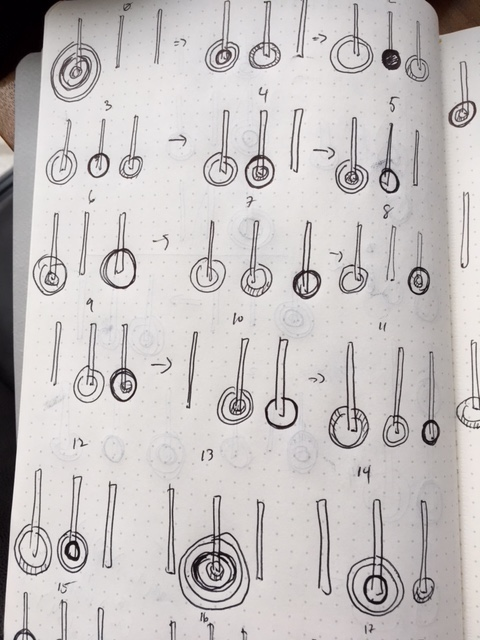
\includegraphics[scale=.5]{towers-1} \\
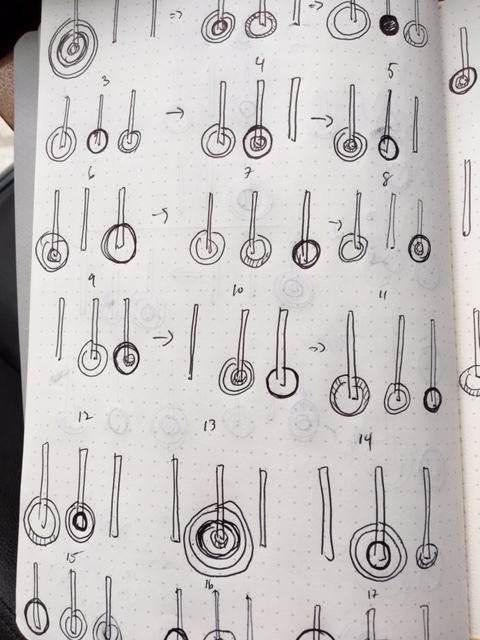
\includegraphics[scale=.5]{towers-2} \\
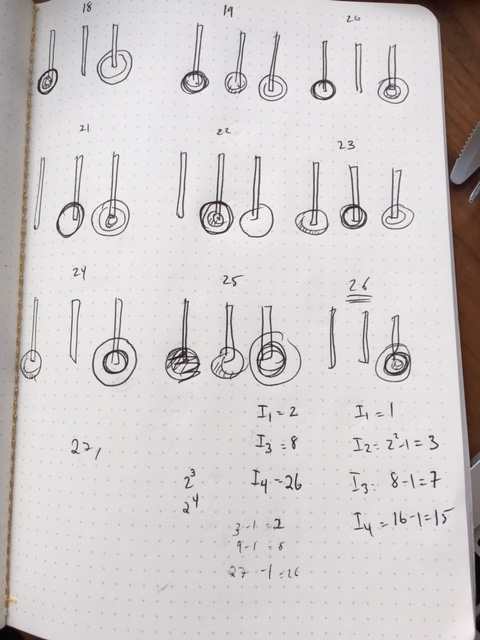
\includegraphics[scale=.5]{towers-3} \\
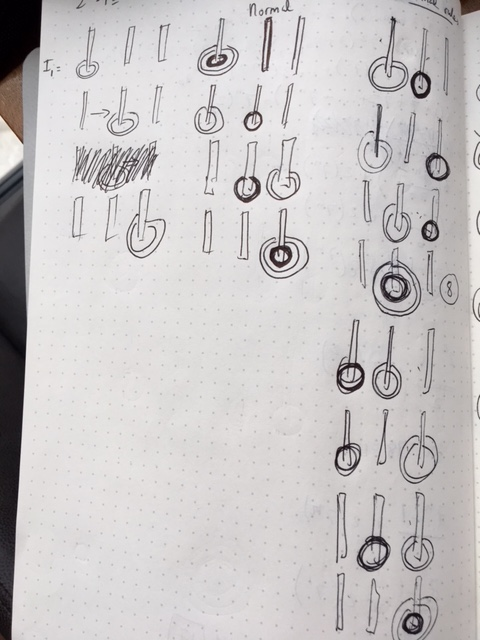
\includegraphics[scale=.5]{towers-4} \\

\subsection{}

Let $a_0 = 0; a_1 = 2$. For $n \ge 2$ then $a_n = (a_{n-1}) + (3^{n-1} * 2)$


\begin{align*}
a_{0} &= 0 \\ 
a_{1} &= 2 \\ 
a_{2} &= (a_{n-1}) + (3^{n-1} * 2) = (a_{2-1}) + (3^{2-1} * 2) = (a_1) + (3^1 * 2) = (2) + (3)(2) = 8 \\ 
a_{3} &= (a_{n-1}) + (3^{n-1} * 2) = (a_{3-1}) + (3^{3-1} * 2) = (a_2) + (3^2 * 2) = (8) + (9)(2) = 26  \\ 
\end{align*}

\subsection{}

\textbf{Solution: } $3^n - 1$

I actually arrived at this solution before calculating the recursive solution, since I guessed the equation based off of the pattern that I noticed.


\end{document}